% Responsable: Jerónimo (relación entre los 4 modelos) — figura central del paper
% Fuentes (12-nov): resultados/m34/ic_costo_meta_zona_12nov.csv, ic_rmax_12nov.csv, m34_grafica_12nov.py
\subsection{Comparación de los cuatro modelos: el precio de la información}\label{sec:comparacion}

La Figura~\ref{fig:precio} junta los dos criterios, con las mismas restricciones
de equidad territorial en los cuatro modelos. El panel A muestra cuántas veces
cuesta el M3, el M4 y el placebo lo que costaría cumplir la misma meta en cada
zona con información perfecta (Modelo 2). El panel B muestra qué fracción del
piso por zona que se podría garantizar con información perfecta logra
garantizar cada modelo con el mismo presupuesto, junto al $r_B$ que exige el
Modelo 1.

\begin{figure}[ht]
\centering
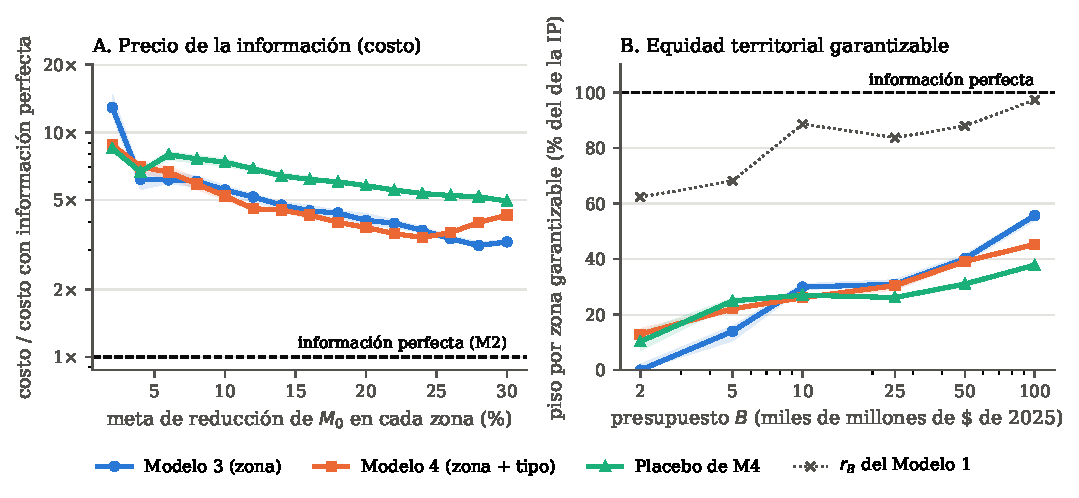
\includegraphics[width=\textwidth]{precio_informacion_12nov}
\caption{El precio de la información, con la equidad territorial de los
Modelos 1 y 2. A: costo de reducir $\Mcero$ en cada zona relativo al costo con
información perfecta (escala logarítmica). B: piso por zona máximo garantizable
como porcentaje del que se garantizaría con información perfecta y el mismo
presupuesto; la línea punteada es el $r_B$ del Modelo 1. Líneas: mediana de las
réplicas; bandas: IC del 95\,\% por \emph{bootstrap}.}
\label{fig:precio}
\end{figure}

Los dos criterios cuentan la misma historia.

\paragraph{1. No saber quién es pobre es caro.} Con metas de hasta el 10\,\% en
cada zona, el Estado que focaliza solo por zona gasta entre \zMtresIPbaja{}
veces lo necesario. El costo de la falta de información es mayor justo donde
están los programas reales, que tienen presupuestos acotados y metas modestas.
Con metas grandes la brecha se reduce, aunque no desaparece: el M3 sigue
costando entre \zMtresIPalta{} veces lo necesario.

\paragraph{2. Sin información individual no se puede prometer la equidad
territorial del Modelo 1.} Con el piso $r_B$ que el Modelo 1 cumple con
información perfecta, M3 y M4 son infactibles en todas las réplicas. El piso
máximo que pueden garantizar va de casi nada con $B=\$2$~mm a entre el 45 y el
56\,\% del de la información perfecta con $B=\$100$~mm (panel B), siempre por debajo de
$r_B$. Un Estado que no sabe quién es pobre no solo gasta más: tampoco puede
asegurar que la reducción de la pobreza llegue a cada zona en la proporción que
podría con información perfecta.

\paragraph{3. La información demográfica vale casi lo mismo que la geográfica.}
Con la meta en cada zona, el M4 cuesta algo menos que el M3 en las metas del 10
al 24\,\% (entre un 4 y un 11\,\% menos), lo mismo en las del 4 al 8\,\% y más en
las del 26 al 30\,\%, y entre un \zPlacMin{} y un \zPlacMax{} menos que un placebo con su
misma partición. La comparación con el placebo muestra que los tipos de
hogar sí contienen información útil, pero que con exigencias territoriales esa
información solo compensa lo que se pierde al no focalizar los indicadores
privados por zona. Sin exigencias territoriales (la sensibilidad de la
Sección~\ref{sec:res34}) la conclusión es otra: el M4 es más barato que el M3,
pero hasta metas del 18\,\% igual de barato que el placebo, de modo que su
ventaja viene de usar celdas más finas.

\paragraph{4. La diferencia es solo de información.} Con un hogar por celda, el
M3 reproduce el costo del M2 con la meta en cada zona y las personas del M1 con
el piso $r_B$, salvo la desviación acotada del ciclo de educación para adultos
(Sección~\ref{sec:diseno}). Por eso las brechas de la Figura~\ref{fig:precio} no
se deben a que los modelos sean distintos: miden el valor de la información
sobre quién es pobre.
